\section{Background}
In this section, we give the necessary backgrounds for buddy memory allocation algorithms and Isabelle/HOL theorem prover.

\subsection{Buddy Allocation Algorithms}
According to the algorithms, free blocks of all possible sizes are maintained in a multilevel list. As a result, it is easy to find a block in requested size if one is available. If there is no block in requested size, allocation operation will search for the first nonempty free list for blocks, whose size is bigger than requested size. Then a large block which is picked from the nonempty free list is split. It is divided into two smaller blocks and each smaller block becomes an unique buddy to the other. If the size of smaller block is still too large, one of the two smaller blocks is split again. The split process stops until one block in requested size appears. Then one of the available blocks is marked as occupied and returned to the requesting application. The others are added to the appropriate free lists.

When a block is deallocated, the algorithms check whether the block can be merged. A split block can only be merged with its unique buddy block, which then reforms the larger block they were split from. Among this process, the algorithms apply a flag bit strategy to quickly check if blocks belonging to the same parent are free, in order to decide whether to merge these blocks into one block. With this way, buddy memory system has small external fragmentation.

To implement buddy allocation algorithms, it applies two important data structures multilevel free linked-list and multilevel free bitmap. The block to be allocated or deallocated is directly picked from the head of linked-list or added into the tail. Bitmap uses 0 and 1 to implement the flag bit strategy. Fig. \ref{fig3} describes a moment in memory system using these two date structures.

\begin{figure}[htbp]
	\centering
	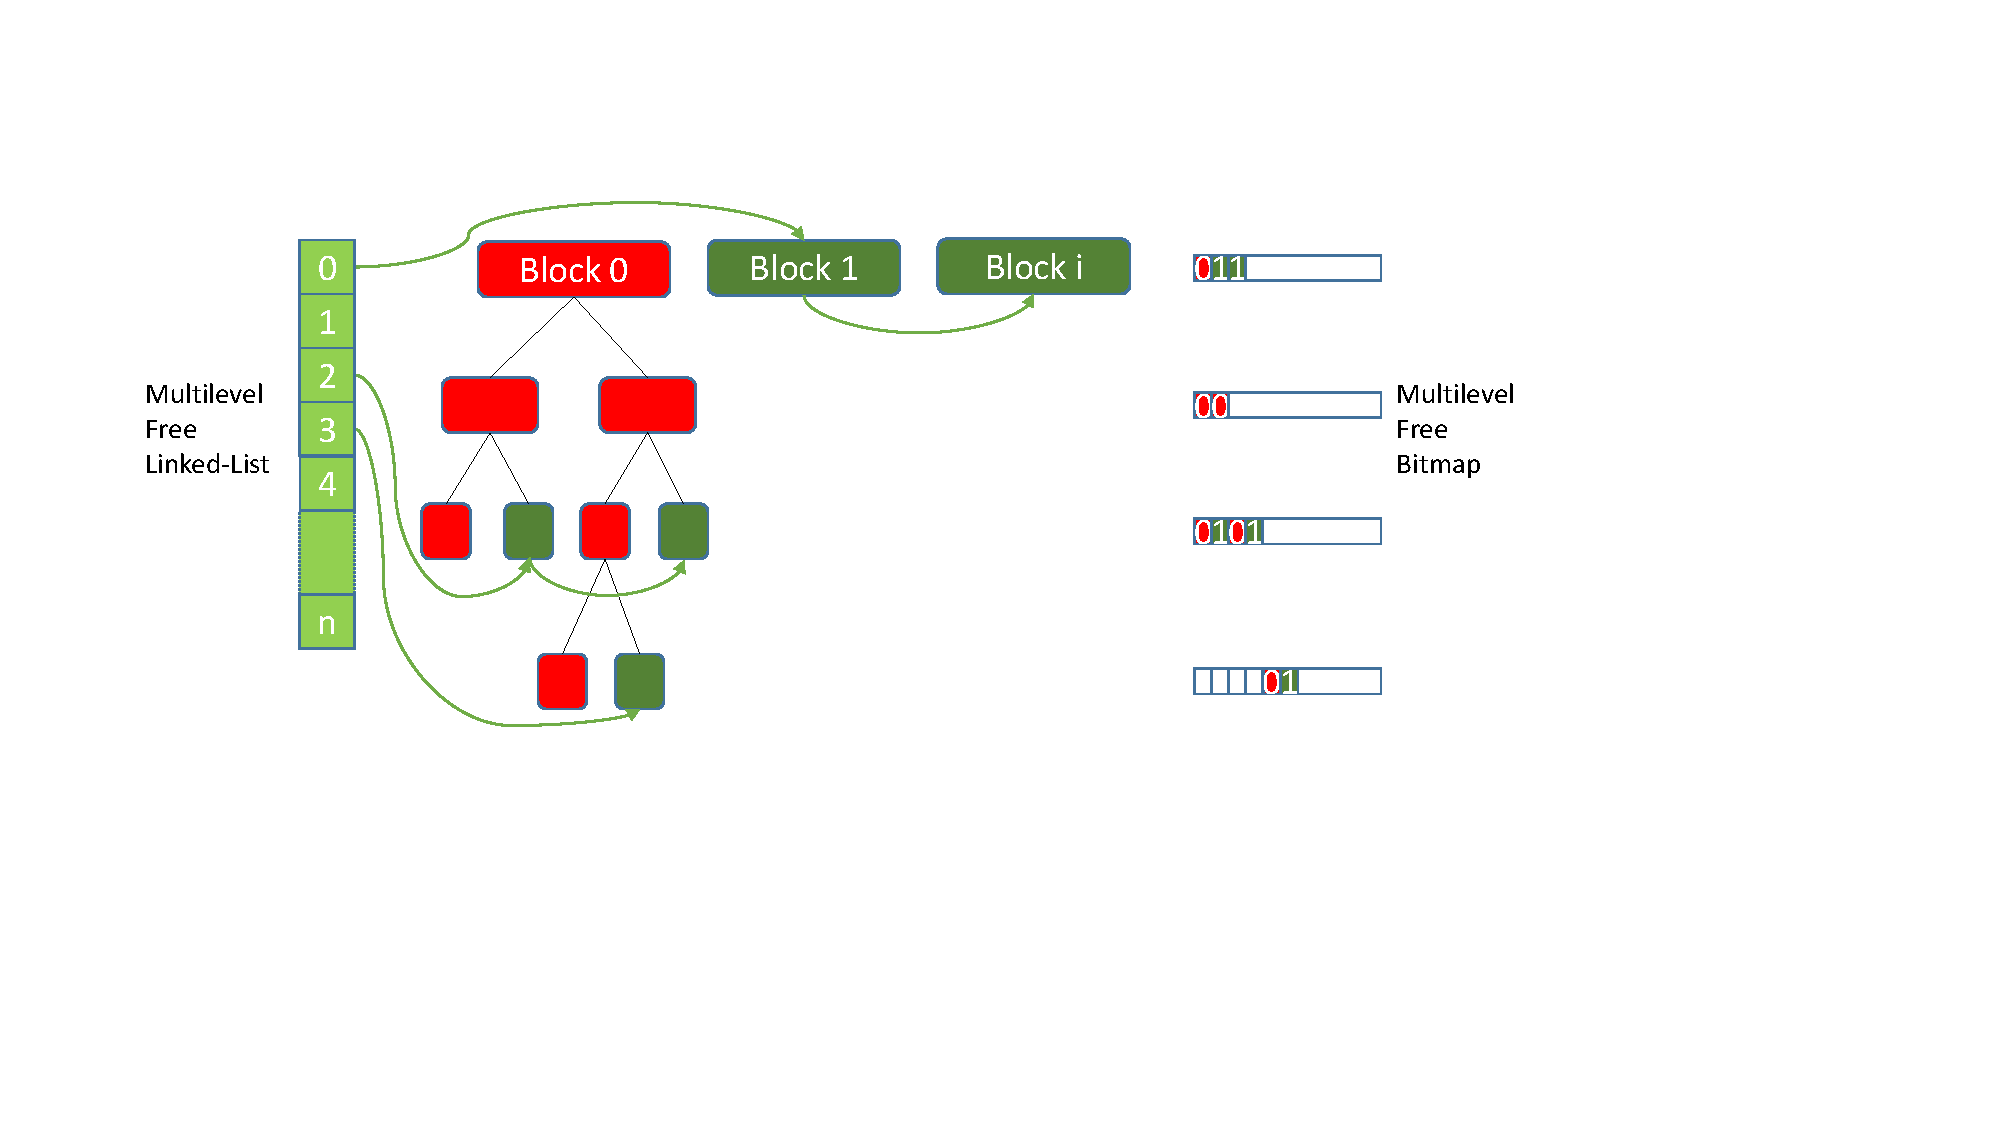
\includegraphics[width=0.5\textwidth]{fig3.pdf}
	\caption{Structures in Buddy Allocation Algorithms}
	\label{fig3}
\end{figure}

\subsection{Isabelle/HOL}
We use interactive theorem prover Isabelle/HOL\cite{reg_Isabelle/HOL} to conduct the specification and verification of the memory management. Isabelle/HOL is a higher order logic theorem prover, using a typed lambda calculus-like functional language for specifications.

Isabelle/HOL includes a specification for simple common types such as naturals (\emph{nat}), integers (\emph{int}) and booleans (\emph{bool}). It also specifies some composed data types like tuples, records, lists and sets that are parametrized with other types. Isabelle provides the interface \emph{datatype} for the creation of user defined types based on type constructors. 

Isabelle provides functions on predefined types to access their members or to provide additional operations over them. In the following we describe those functions that we use along this work. A tuple is denoted as (\emph{$t_1$} $\times$ \emph{$t_2$}), projection functions \emph{fst} and \emph{snd} respectively return elements $t_1$ and $t_2$. Lists are defined as a datatype with an empty construct denoted with \emph{NIL} or $[]$, and a concatenation construct denoted with $\#$, where $x\#xs$ adds $x$ to the front of $xs$. The $i$th component of a list $as$ is written as $as!i$. Isabelle/HOL provides functions for definite and indefinite descriptions. Definitive description is represented by $THE\ x.\ P\ x$ and returns the element uniquely described by the predicate $P$, else it returns and undefined value. Indefinite description is represented by $SOME\ x.\, P\ x$, selecting a random element from the predicate $P$ that must describe at least one element, else it returns an arbitrary value.

Isabelle/HOL allows user to create non-recursive specifications using the command \emph{definition}, and to create recursive specifications using commands \emph{primrec} and \emph{recursive}.
